\chapter{Mon corps}\label{ch:g1:my-body}

Mets-toi devant un miroir et fais un signe~: c'est tout un corps
vivant qui te répond. Il grandit depuis avant ta naissance, il plie
à certains endroits et pas à d'autres, et il est à toi pour la vie.
Il est temps de le regarder comme nous avons regardé le chat et la
pâquerette --- partie par partie.

\section{Les parties de mon corps}

\begin{definition}[Les parties du corps humain]\label{def:g1:my-body:parts}
Le corps humain a trois parties principales~:
\begin{enumerate}
  \item la \emph{tête}\index{tête}, qui porte le visage, les yeux,
        les oreilles, le nez et la bouche~;
  \item le \emph{tronc}\index{tronc (corps)}, le milieu du corps ---
        poitrine, ventre et dos~;
  \item les \emph{membres}\index{membre}~: deux \emph{bras}\index{bras}
        terminés par des mains, deux \emph{jambes}\index{jambe}
        terminées par des pieds.
\end{enumerate}
La tête est posée sur le \emph{cou}\index{cou}, qui la relie au
tronc.
\end{definition}

\begin{omfigure}
\begin{tikzpicture}
  \node[anchor=south west, inner sep=0] (img) at (0,0)
    {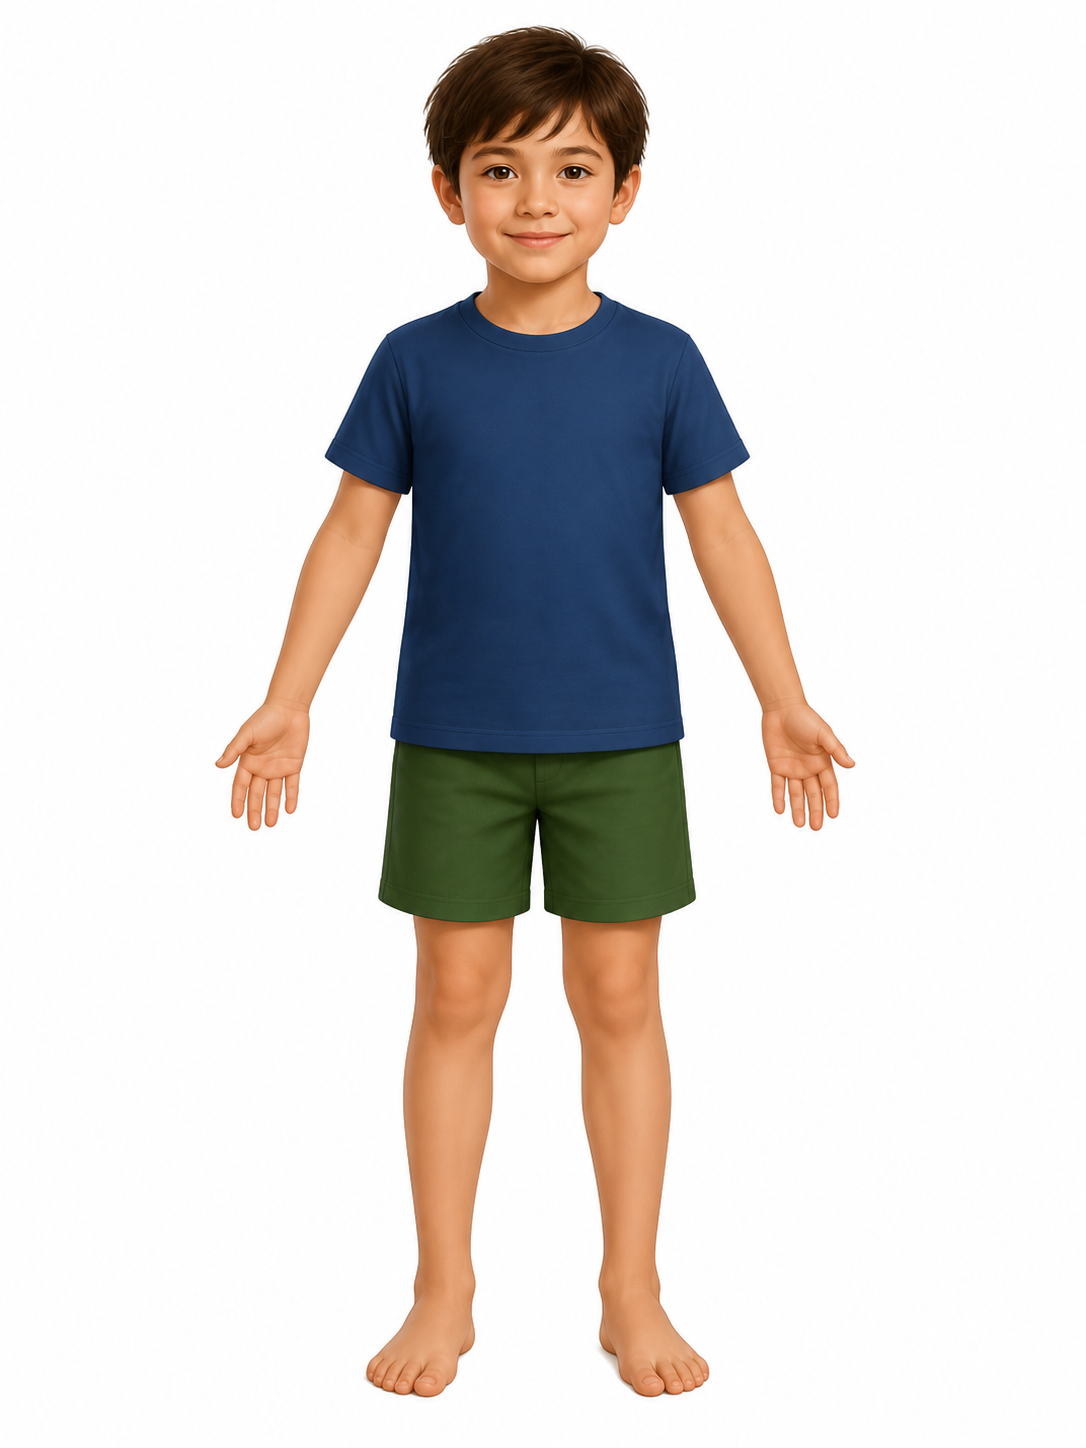
\includegraphics[width=0.42\linewidth]{images/book1/ai/fig-child-standing.png}};
  \begin{scope}[x={(img.south east)}, y={(img.north west)},
      every node/.style={font=\small}]
    \draw[omDef, thick] (0.57,0.90) -- (0.76,0.92) node[right] {tête};
    \draw[omDef, thick] (0.53,0.80) -- (0.76,0.83) node[right] {cou};
    \draw[omDef, thick] (0.58,0.62) -- (0.78,0.66) node[right] {tronc};
    \draw[omDef, thick] (0.74,0.46) -- (0.86,0.38)
      node[below, align=center] {bras et\\ main};
    \draw[omDef, thick] (0.60,0.18) -- (0.78,0.14)
      node[right, align=left] {jambe et\\ pied};
  \end{scope}
\end{tikzpicture}

{\small Les trois parties principales du corps~: tête, tronc et
quatre \omterm{def:g1:my-body:parts}{membres} --- avec le cou qui relie la tête au tronc.}
\end{omfigure}

\begin{example}[Le même plan que le chat~?]\label{ex:g1:my-body:cat}
Compare-toi au chat~: une tête, un corps, quatre \omterm{def:g1:my-body:parts}{membres} --- le plan
se ressemble. Mais le chat marche sur ses quatre pattes~; toi, tu
tiens debout sur deux \omterm{def:g1:my-body:parts}{jambes} et tu gardes deux \omterm{def:g1:my-body:parts}{bras} libres pour
porter, dessiner et faire signe. Et là où le chat a une queue, tu
n'en as pas.
\end{example}

\section{Plier~: les articulations}

\begin{definition}[Articulation]\label{def:g1:my-body:joint}
Une \emph{articulation}\index{articulation} est un endroit où le
corps peut plier ou tourner. Le \emph{coude}\index{coude} plie le
\omterm{def:g1:my-body:parts}{bras}, le \emph{genou}\index{genou} plie la \omterm{def:g1:my-body:parts}{jambe},
l'\emph{épaule}\index{épaule} fait tourner tout le \omterm{def:g1:my-body:parts}{bras}, le
\emph{poignet}\index{poignet} et la \emph{cheville}\index{cheville}
plient la main et le pied. Entre deux articulations, le corps reste
droit.
\end{definition}

\begin{omfigure}
\begin{tikzpicture}[scale=1.0]
  % straight arm
  \draw[very thick] (0,0) -- (2.0,0);
  \draw[very thick] (2.0,0) -- (3.8,0);
  \fill[omThm] (2.0,0) circle (0.1);
  \fill[omDef!60] (0,0) circle (0.1);
  \draw[thick, fill=omDef!8] (4.0,0) circle (0.18);
  \node[below, font=\small] at (1.9,-0.3) {bras tendu};
  % bent arm
  \begin{scope}[xshift=6.6cm]
    \draw[very thick] (0,0) -- (2.0,0);
    \draw[very thick] (2.0,0) -- (3.1,1.45);
    \fill[omThm] (2.0,0) circle (0.1);
    \fill[omDef!60] (0,0) circle (0.1);
    \draw[thick, fill=omDef!8] (3.22,1.6) circle (0.18);
    \node[below, font=\small] at (1.9,-0.3) {bras plié au coude};
    \draw[omThm] (2.05,0.12) -- (1.55,0.8)
      node[above left, font=\small, omThm] {l'articulation plie};
  \end{scope}
  \node[font=\small] at (1.0,1.4) {épaule};
  \draw[omDef!60] (0.05,0.12) -- (0.55,1.15);
\end{tikzpicture}

{\small Le \omterm{def:g1:my-body:parts}{bras} ne plie qu'à ses \omterm{def:g1:my-body:joint}{articulations}~: l'\omterm{def:g1:my-body:joint}{épaule} (en bleu)
et le \omterm{def:g1:my-body:joint}{coude} (en rouge). Entre les deux, il reste droit.}
\end{omfigure}

\begin{example}[Essaie~: la marche à genoux raides]\label{ex:g1:my-body:stiff}
Essaie de marcher sans plier les genoux. Ça marche --- tout juste
--- à petits pas raides de canard. Essaie maintenant de ramasser un
crayon par terre sans plier ni genoux, ni hanches, ni dos. Ce sont
les \omterm{def:g1:my-body:joint}{articulations} qui rendent les mouvements du corps souples,
rapides et faciles.
\end{example}

\begin{remark}[Droite et gauche]\label{rem:g1:my-body:sides}
Le corps a deux côtés, droit et gauche, presque comme dans un
miroir~: un \omterm{def:g1:my-body:parts}{bras} et une \omterm{def:g1:my-body:parts}{jambe} de chaque côté, un œil et une oreille
de chaque côté de la tête. Savoir reconnaître ta main droite de ta
main gauche fait aussi partie de la connaissance du corps --- cela
dit aux autres de quel côté tu parles.
\end{remark}

\section{Mon corps grandit}

\begin{proposition}[Grandir]\label{prop:g1:my-body:growth}
Le corps d'un enfant \emph{grandit}\index{grandir}~: il devient plus
haut et plus lourd, année après année, jusqu'à la taille adulte.
Grandir est lent et régulier --- trop lent pour se sentir, facile à
mesurer.
\end{proposition}
\admitted

\begin{example}[Les traits sur le montant de la porte]\label{ex:g1:my-body:doorframe}
Mets-toi contre le montant de la porte~; un adulte marque ta taille
au crayon. Recommence quelques mois plus tard~: le nouveau trait est
plus haut~! Tu ne t'es jamais senti grandir, mais les deux traits,
l'un au-dessus de l'autre, le montrent clairement.
\end{example}

\begin{omfigure}
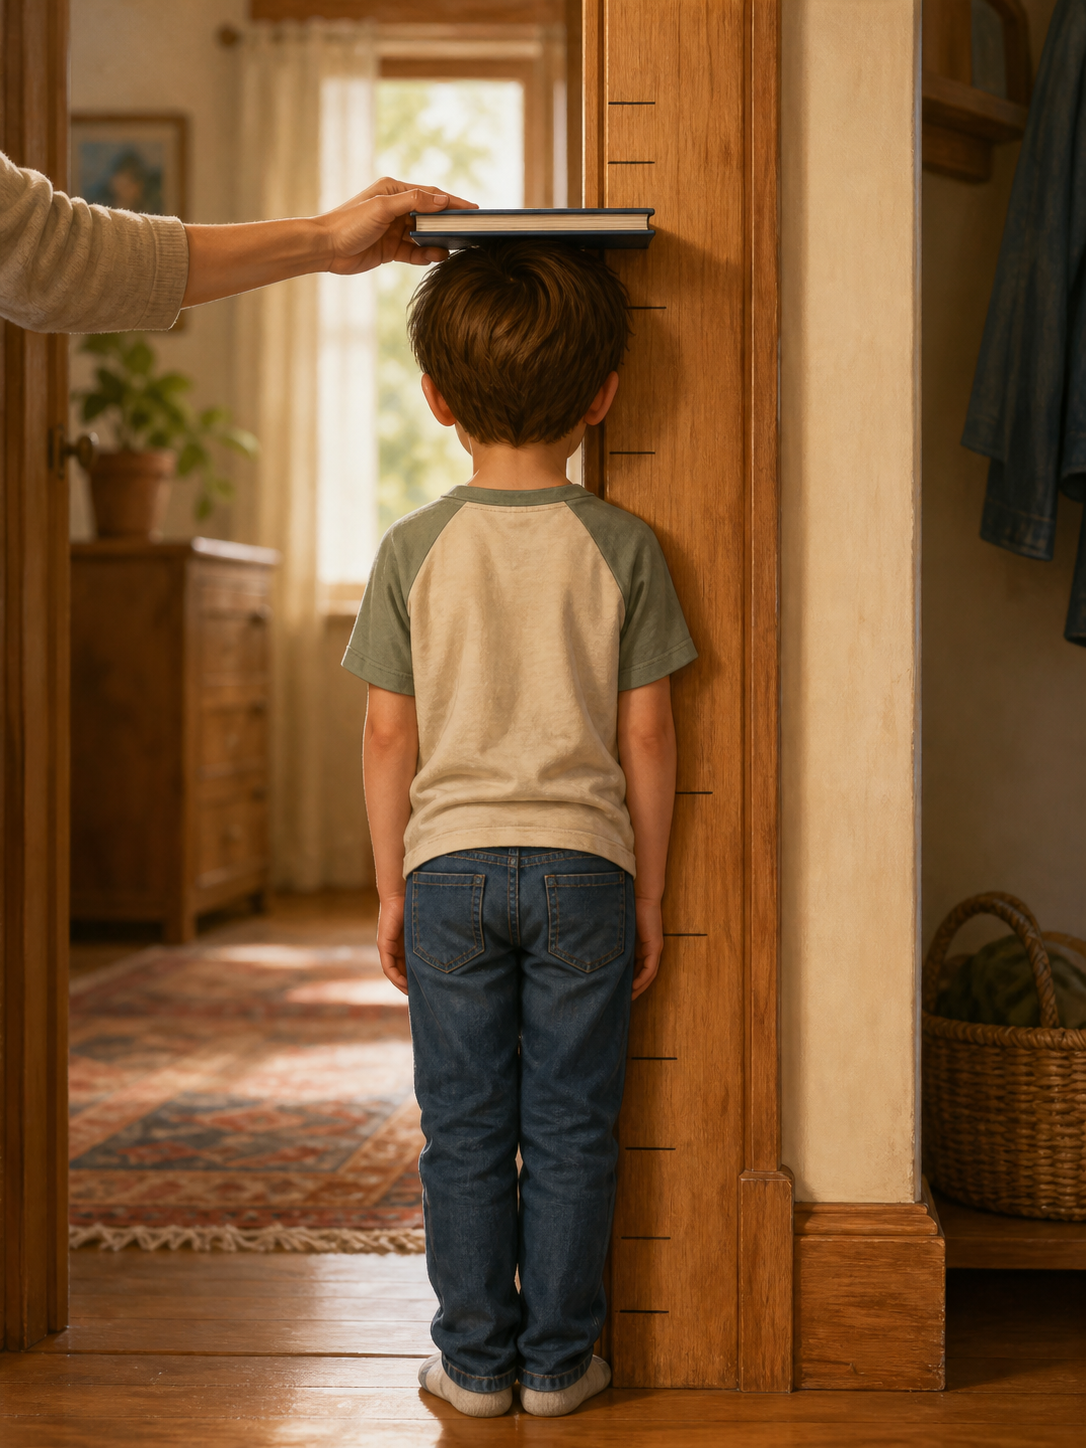
\includegraphics[width=0.46\linewidth]{images/book1/ai/g1-body-doorframe.png}

{\small Jour de mesure au montant de la porte~: le livre bien plat
amène le sommet de la tête juste au bois.}
\end{omfigure}

\begin{method}[Mesurer ma taille]\label{met:g1:my-body:measure}
\begin{enumerate}
  \item Enlève tes chaussures~;
  \item tiens-toi droit, dos et talons contre le mur, le regard
        devant toi~;
  \item quelqu'un pose un livre plat sur ta tête, bien horizontal,
        touchant le mur~;
  \item marque l'endroit sous le livre, et écris la date à côté.
\end{enumerate}
Mesurés de la même façon chaque fois, les traits sont fiables ---
et comparables.
\end{method}

\begin{remark}[Chaque corps est différent]\label{rem:g1:my-body:different}
Dans une même classe, certains enfants sont plus grands, d'autres
plus petits~; certains grandissent plus tôt, d'autres plus tard.
Tout cela est normal. Les corps sont comme les visages~: bâtis sur
le même plan, et tous différents. Les traits sur ton montant de
porte sont les tiens --- ils ne servent pas à faire la course avec
le voisin.
\end{remark}

\section{Exercices}

\begin{exercise}[$\star$]\label{exo:g1:my-body:1}
Nomme les trois parties principales du corps humain. Qu'est-ce qui
relie la tête au tronc~?
\end{exercise}

\begin{exercise}[$\star$]\label{exo:g1:my-body:2}
Où se termine chaque \omterm{def:g1:my-body:parts}{membre} --- qu'y a-t-il au bout d'un \omterm{def:g1:my-body:parts}{bras}, et au
bout d'une \omterm{def:g1:my-body:parts}{jambe}~?
\end{exercise}

\begin{exercise}[$\star$]\label{exo:g1:my-body:3}
Quelle \omterm{def:g1:my-body:joint}{articulation} plie~: (a) le \omterm{def:g1:my-body:parts}{bras} en son milieu~? (b) la \omterm{def:g1:my-body:parts}{jambe}
en son milieu~? (c) la main au bout du \omterm{def:g1:my-body:parts}{bras}~?
\end{exercise}

\begin{exercise}[$\star$]\label{exo:g1:my-body:4}
Touche ton oreille droite avec ta main gauche. Quelles \omterm{def:g1:my-body:joint}{articulations}
ton \omterm{def:g1:my-body:parts}{bras} vient-il d'utiliser~? Nomme-en au moins deux.
\end{exercise}

\begin{exercise}[$\star$]\label{exo:g1:my-body:5}
Dans \cref{ex:g1:my-body:cat}, trouve un point commun entre ton
corps et celui du chat, et deux différences.
\end{exercise}

\begin{exercise}[$\star$]\label{exo:g1:my-body:6}
Pourquoi la personne qui aide dans \cref{met:g1:my-body:measure}
pose-t-elle un livre plat sur ta tête au lieu de regarder simplement~?
\end{exercise}

\begin{exercise}[$\star$]\label{exo:g1:my-body:7}
Deux traits sur le montant de la porte~: celui de l'an dernier, et
celui d'aujourd'hui, un peu plus haut. Que montrent ces traits~?
L'as-tu senti se produire~?
\end{exercise}

\begin{exercise}[$\star$]\label{exo:g1:my-body:8}
À toi d'essayer~: fais la marche à genoux raides de
\cref{ex:g1:my-body:stiff}, puis essaie d'applaudir sans plier les
\omterm{def:g1:my-body:joint}{coudes}. Quels gestes de tous les jours ont finalement besoin
d'\omterm{def:g1:my-body:joint}{articulations}~?
\end{exercise}

\begin{exercise}[$\star\star$]\label{exo:g1:my-body:9}
Mia est la plus petite de sa classe et cela l'inquiète. Que lui
répond \cref{rem:g1:my-body:different}~?
\end{exercise}

\begin{exercise}[$\star\star$]\label{exo:g1:my-body:10}
Un pantin fait d'un seul bâton de bois ne peut pas s'asseoir sur une
chaise. Où couperais-tu le bâton et où ajouterais-tu des points de
rotation pour qu'il puisse s'asseoir~? Nomme les \omterm{def:g1:my-body:joint}{articulations} du
corps que tes coupures imitent.
\end{exercise}
